
\begin{frame}{Dictionary-based manifold learning}
\begin{algorithm}[H]
\caption{\tsalg(Dataset $\mathcal D$, dictionary $g$)}
\begin{algorithmic}[1]
\STATE Compute Jacobian $d g (n) \in \mathbb R^{P \times B} \; \forall  n \in [N]$
\STATE Normalize $\|d g^p \|_F = \sqrt{N} \; \forall  p \in [P]$
\STATE Estimate tangent basis $T_{\mathcal M}(n) \in \mathbb R^{D \times B} \; \forall  n \in [N]$
\STATE Project $d_\M g (n) = {T_{\mathcal M} (n)}^T d g (n) \; \forall  n \in [N]$
\STATE  $\hat \beta \gets \arg \min_{\beta \in \mathbb R^{N \times P \times D}} J_\lambda ( d_\M g ([N]),\beta)$ (Group Lasso)
\STATE {\bf Output} $S= \supp \hat  \beta$ 
\end{algorithmic}
\end{algorithm}
\begin{itemize}
\item $J_\lambda (X, \beta) =  \frac{1}{2}\sum_{n=1}^N \| I_D  - X_{n..} \beta_{n..}\|_F^2+\frac{\lambda}{\sqrt{DN}} \sum_{p=1}^P \|\beta_{.p.}\|_F. $
\item Optimize with FISTA
\item Locate region on regularization path with $|S| = D$ using binary search
\end{itemize}
\end{frame}


\begin{frame}{Estimating tangent spaces using local PCA}
\begin{columns}
\begin{column}{0.35\textwidth}
\begin{itemize}
    \item First, perform a nearest neighbor search around $\xi = \mathcal D(n) \in \mathcal M$
    \item Then, estimate $ T_{\mathcal M}(n) $ using the top singular vectors $[x^1, \dotsc x^D]$ of the centered neighbors
\end{itemize}
\end{column}
\begin{column}{0.6\textwidth}
\begin{figure}
    \includegraphics[width=2.5in]{img/tangentspaces.png}
    \caption*{A neighborhood and tangent space plotted in top global PCA coordinates}
\end{figure}
\end{column}
\end{columns}


\end{frame}

\begin{frame}{Gradients}
\begin{itemize}
    \item We can compute dihedral angle gradients with autograd
    \item We then project $d_{\mathcal M} g (n) = (T_{\mathcal M} (n))^T d g (n)$
\end{itemize}
\small
\begin{figure}[!htp]
    \centering
    \begin{tabular}{p{2.5cm}p{2.5cm}p{2.5cm}p{2.5cm}}
        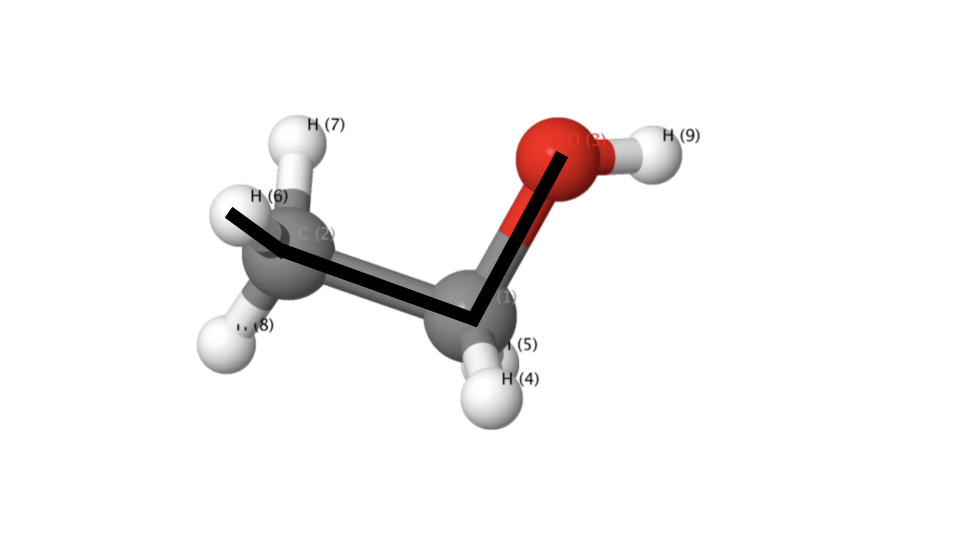
\includegraphics[width=0.25\textwidth, trim={2cm 3cm 5cm 0cm}, clip]{img/ethanol_g0.png} &
        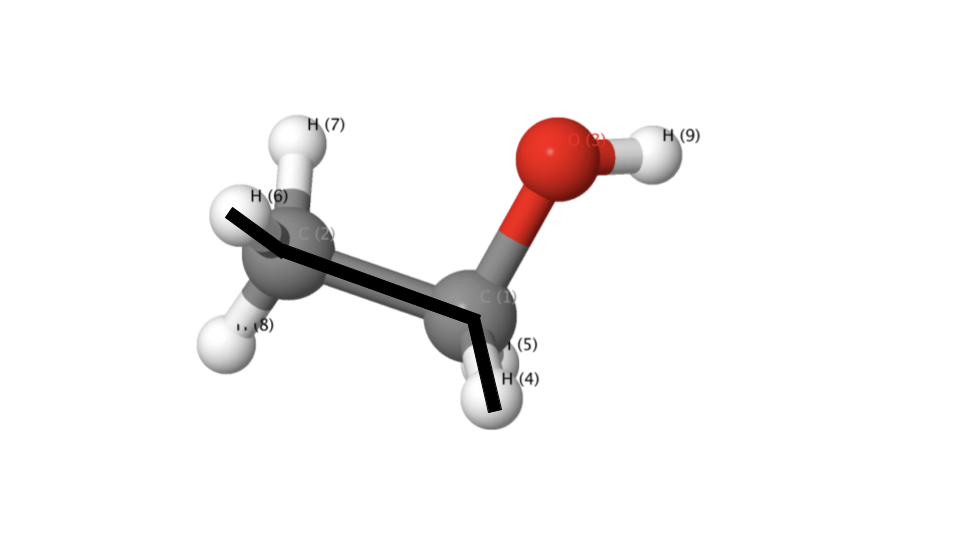
\includegraphics[width=0.25\textwidth, trim={2cm 3cm 5cm 0cm}, clip]{img/ethanol_g1.png} &
          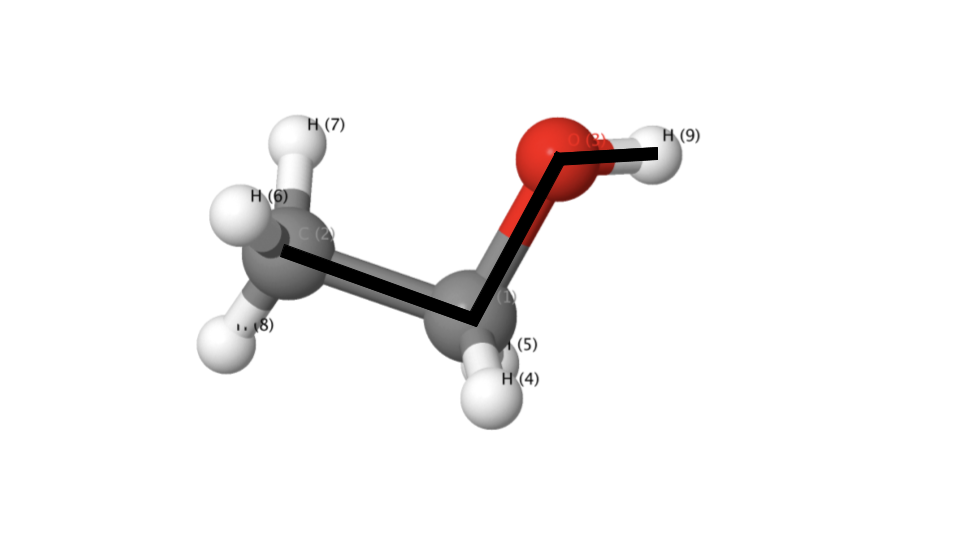
\includegraphics[width=0.25\textwidth, trim={2cm 3cm 5cm 0cm}, clip]{img/ethanol_g2.png} &
          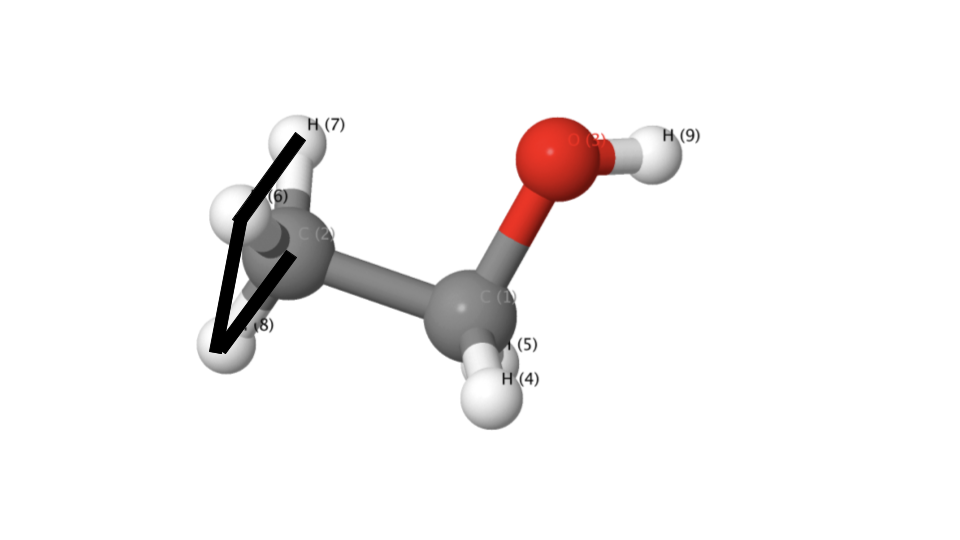
\includegraphics[width=0.25\textwidth, trim={2cm 3cm 5cm 0cm}, clip]{img/ethanol_g3.png}  \\
        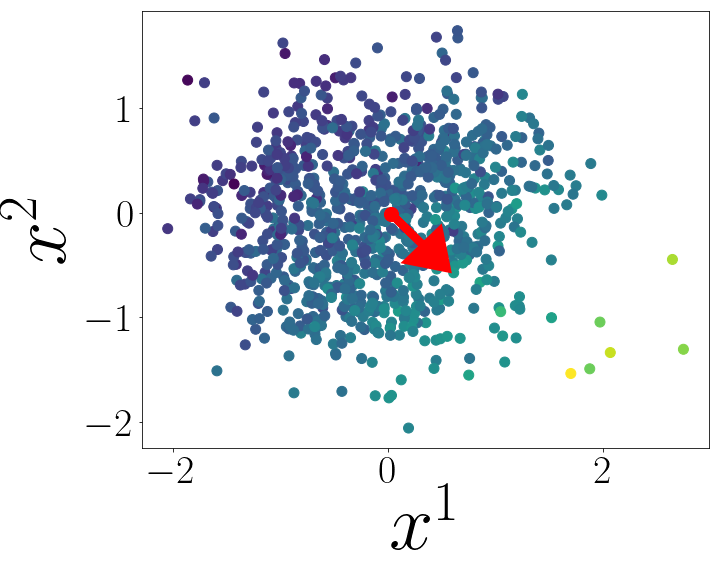
\includegraphics[width=0.2\textwidth]{img/tangent_0.png} &
        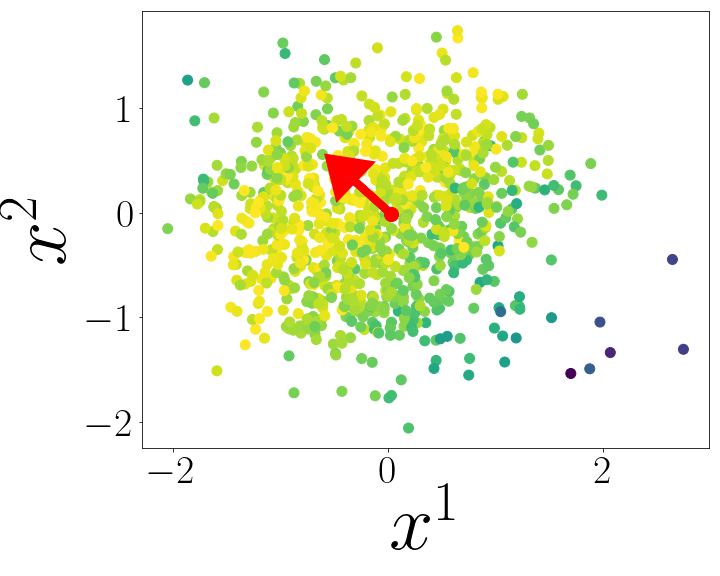
\includegraphics[width=0.2\textwidth]{img/tangent_1.png} &
         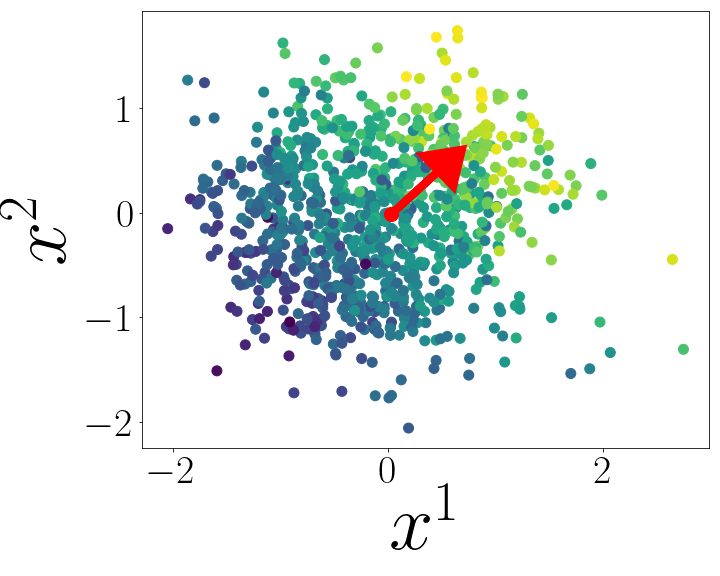
\includegraphics[width=0.2\textwidth]{img/tangent_2.png}  &
          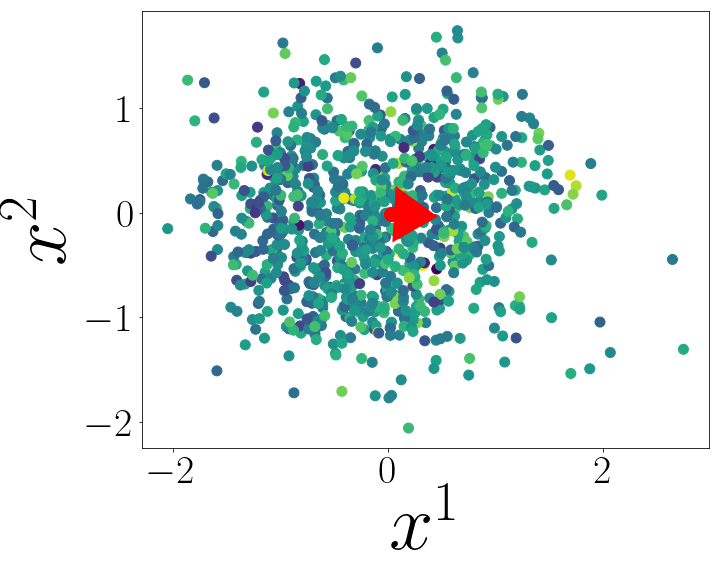
\includegraphics[width=0.2\textwidth]{img/tangent_3.png} 
    \end{tabular}
    %\vspace{-2cm}
    \caption*{ Gradients $dg^p = \frac{\partial g^p }{\partial x^d} $ of four dihedral angles $g^p:\mathcal M \to \mathbb R$ with respect to coordinates $x^1 \dots x^D$ of tangent space $\mathcal {T}_{\mathcal M} (n)$}
\end{figure}
\end{frame}


\begin{frame}{Normalization}
\begin{itemize}
    \item We normalize $d g^p(n)= \frac{\sqrt{N} d g^p(n)}{  \|d g^p([N])\|_F}$ prior to projection to favor gradient fields which are more tangent to the manifold
\end{itemize}
\begin{figure}[!htp]
    \centering
    \begin{tabular}{ccc}
        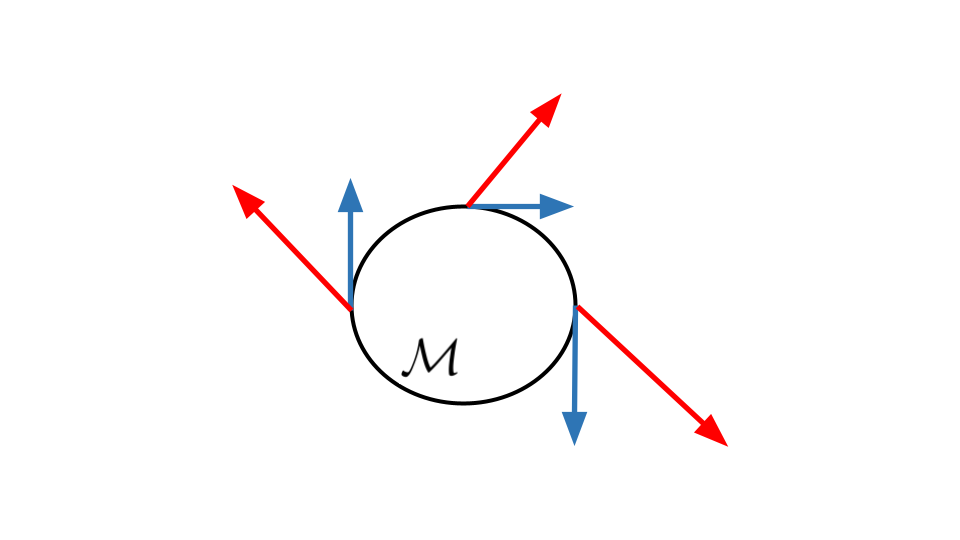
\includegraphics[width=0.3\textwidth, trim={3cm 2cm 5cm 3cm}, clip]{img/raw.png} &
        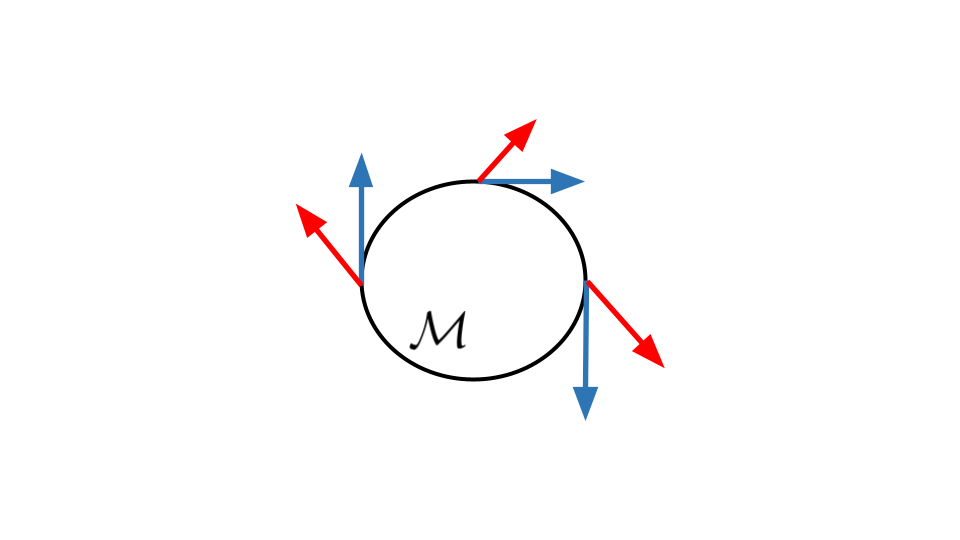
\includegraphics[width=0.3\textwidth, trim={3cm 2cm 5cm 3cm}, clip]{img/norm.png} &
          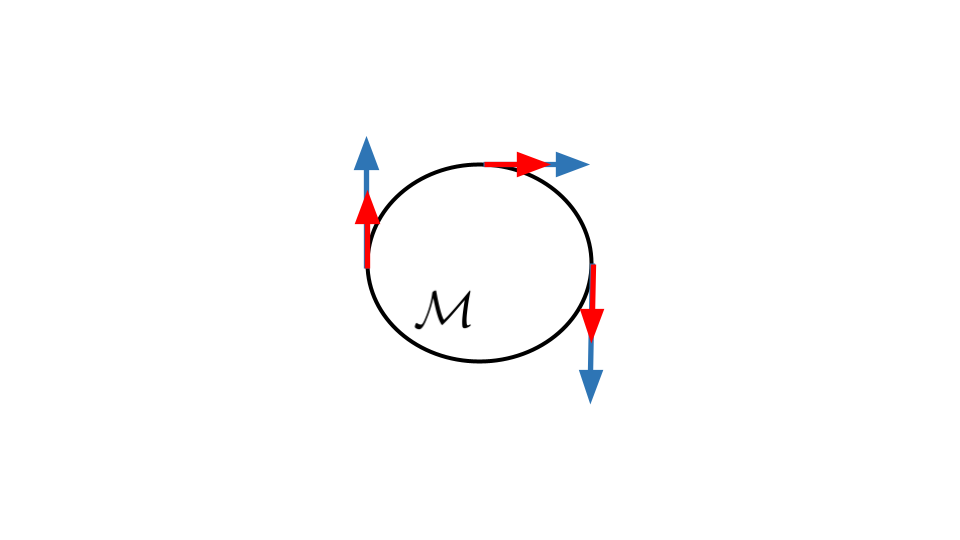
\includegraphics[width=0.3\textwidth, trim={3cm 2cm 5cm 3cm}, clip]{img/proj.png}  \\
           \centering
        $dg$ &
         \centering
       $dg$ (normalized) &
        \centering
        $d_{\mathcal M} g$
    \end{tabular}
    \caption*{Gradients of example functions \textcolor{red}{$g^1$} and \textcolor{blue}{$g^2$} for $B = 2, D = 1$}
\end{figure}
\begin{itemize}
    \item Note: gradients of dihedral angles w.r.t. planar angles are not well-defined and so we use $dg = d_{\mathbb R^{3N_a}} g (d_{\mathbb R^{3N_a}} \alpha)^{\dagger_{3N_a - 7}}$
\end{itemize}
\end{frame}

\begin{frame}{Results}
\begin{figure}[!htp]
    \centering
    \begin{tabular}{p{3cm}p{3cm}p{3cm}}
        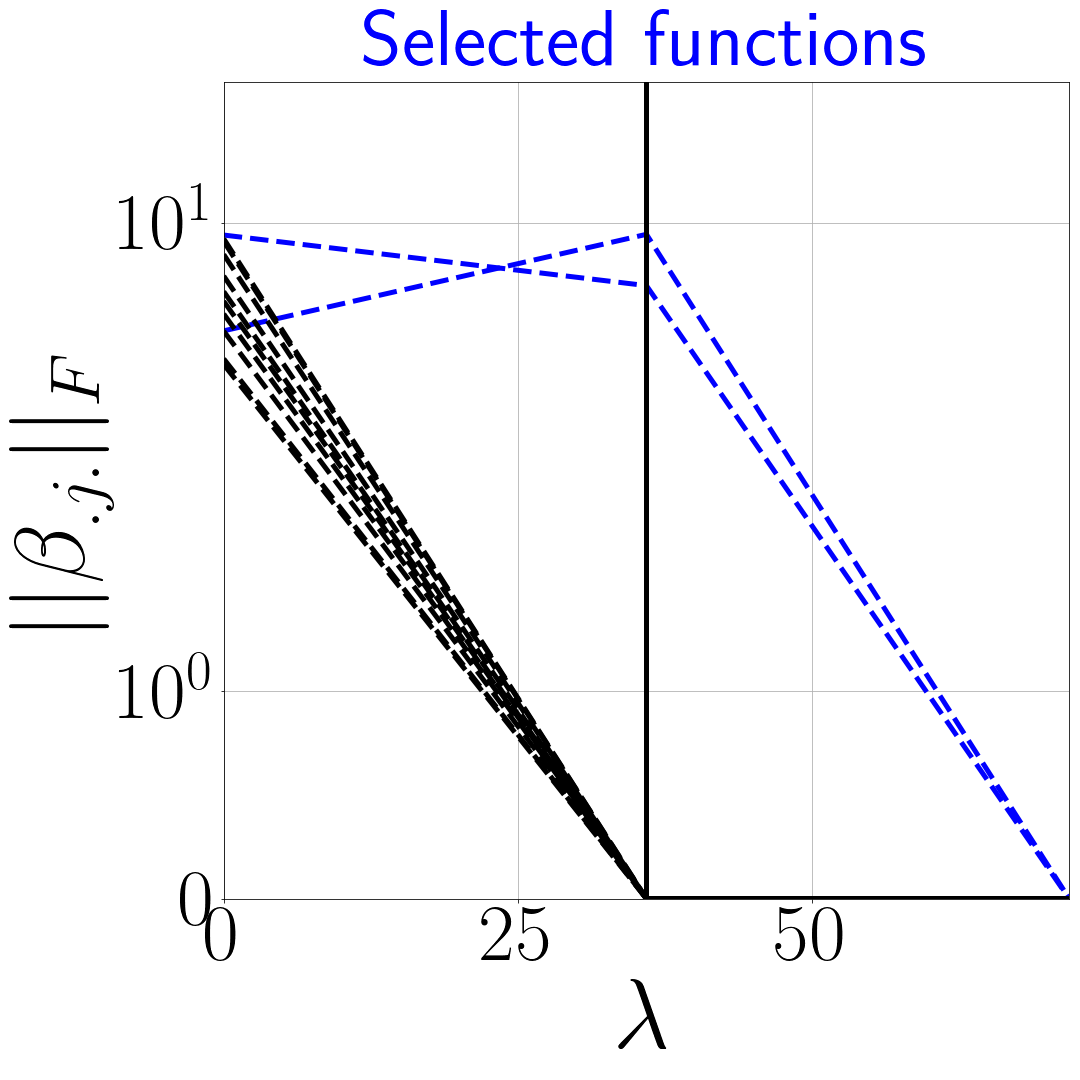
\includegraphics[width=0.2\textwidth]{img/reg_small.png} &
        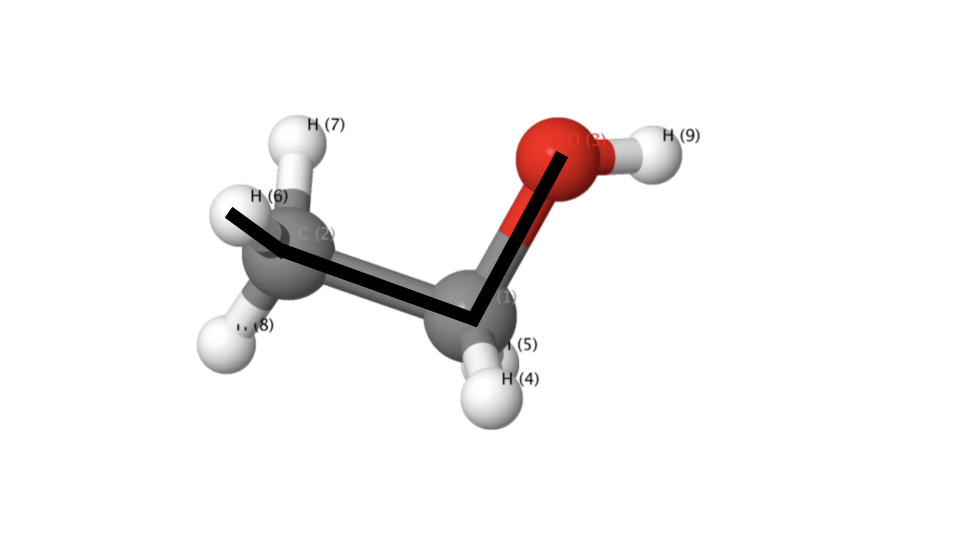
\includegraphics[width=0.35\textwidth, trim={3cm 0cm 0cm 4cm}, clip]{img/ethanol_g0.png} &
          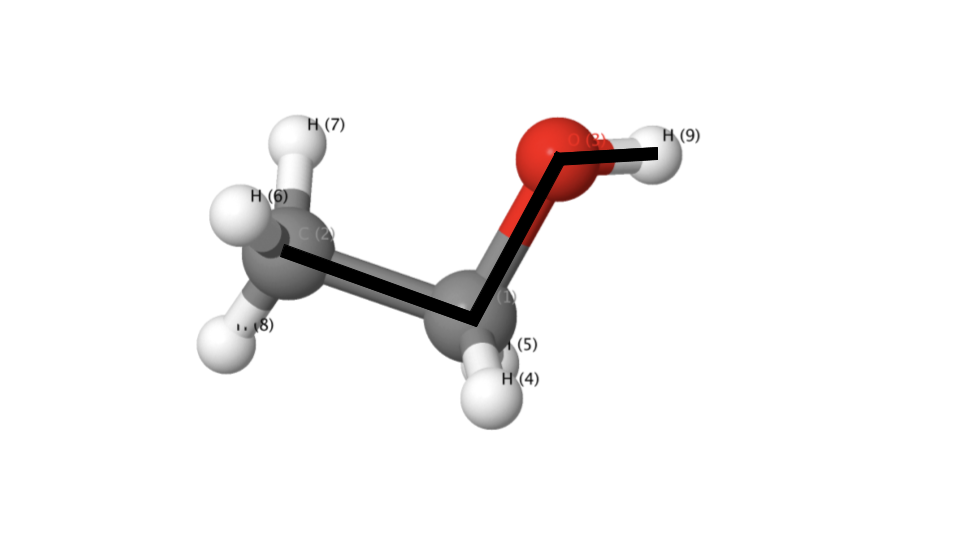
\includegraphics[width=0.35\textwidth, trim={3cm 0cm 0cm 4cm}, clip]{img/ethanol_g2.png}  \\
        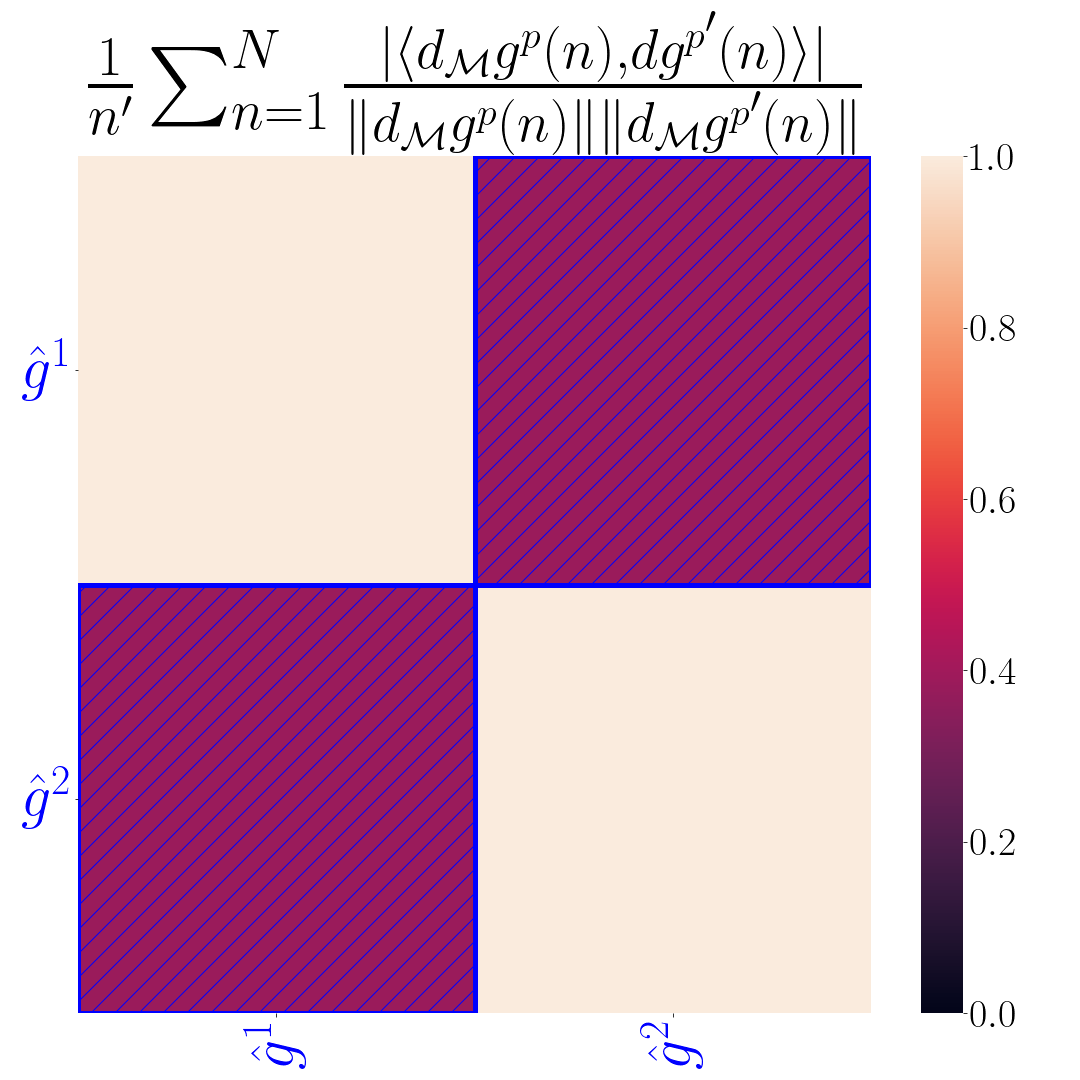
\includegraphics[width=0.2\textwidth, trim={0cm 0cm 3cm 0cm}, clip]{img/cosines_sellasso_small.png} &
        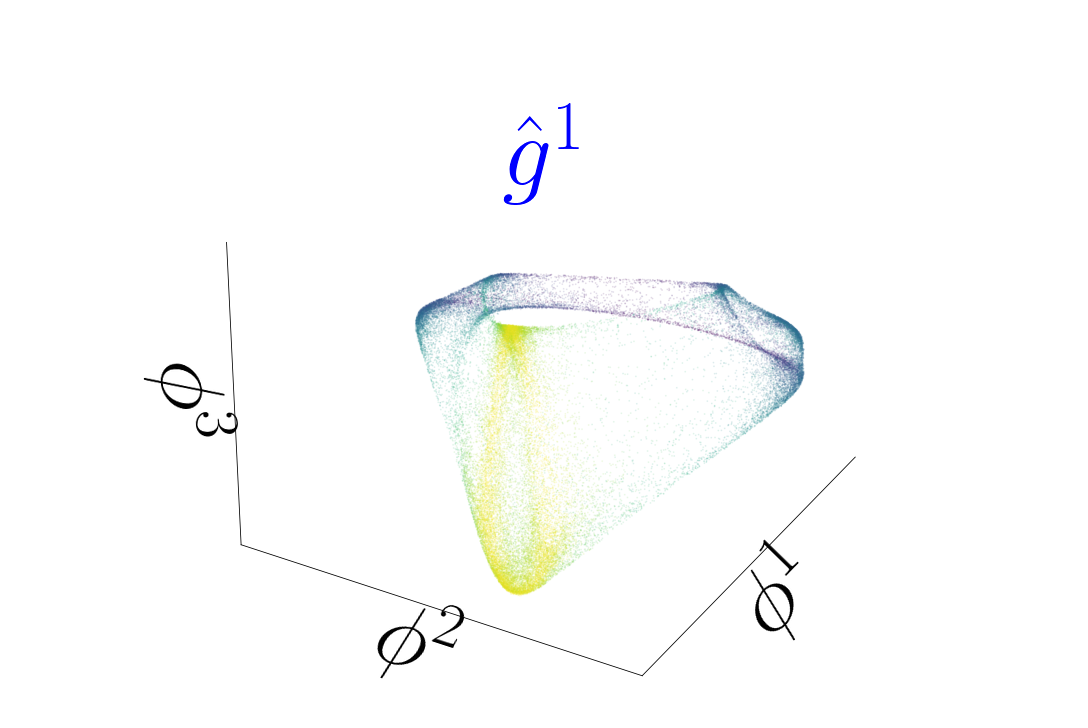
\includegraphics[width=0.35\textwidth, trim={3cm 0cm 0cm 3cm}, clip]{img/ethanol_small_embedding_0.png} &
          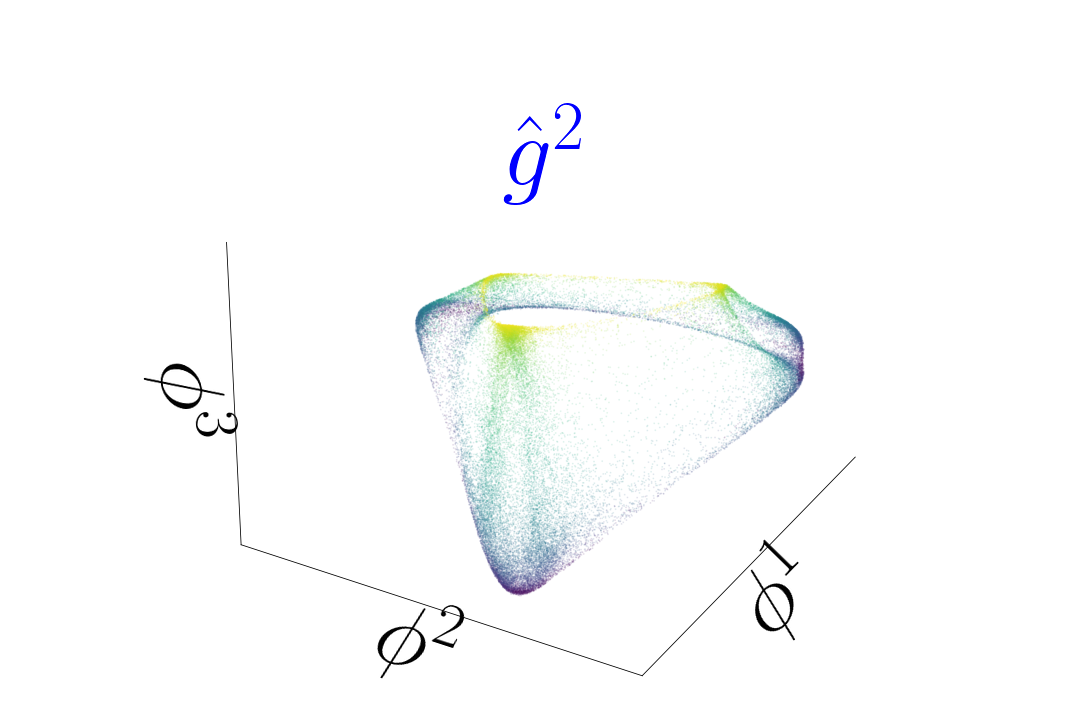
\includegraphics[width=0.35\textwidth, trim={3cm 0cm 0cm 3cm}, clip]{img/ethanol_small_embedding_1.png} 
    \end{tabular}
    %\vspace{-2cm}
    \caption*{Results for one replicate with $P=12$ dictionary functions implicitly defined by the ethanol bond diagram}
\end{figure}
\end{frame}
% 1 
